\documentclass{article}
\usepackage{graphicx}
\usepackage[spanish]{babel}
\usepackage[letterpaper,portrait,margin=1in]{geometry}
\usepackage{hyperref}
\usepackage[section]{placeins}
\usepackage{xurl}
\title{}
\author{}
\date{}
\begin{document}
%\maketitle

\tableofcontents
\setcounter{page}{2}
\newpage

\section{Introducción} 
El surgimiento de grandes cantidades de datos informáticos en el mundo ha propiciado también el invento de nuevas técnicas y metodologías
que permiten su análisis aprovechando la gran capacidad de cómputo que hay hoy en día los equipos. La Minería de Datos es
un área de la Inteligencia Artificial que permite el descubrimiento de elementos ocultos en un conjunto de datos. Esta área
nos proporciona diferentes aplicaciones que van desde la Medicina hasta la Economía, ejemplo de ello: redes neuronales ocupadas
para la detección de diferentes enfermedades, reconocimiento facial, autos autónomos, ventas en línea como Amazon o Mercado Libre. \\

\noindent Los algoritmos que se han implementado para hacer este tipo de análisis permiten a las empresas, organizaciones y comunidades tener
un indicio de lo que está sucediendo o de lo que podría suceder, ahorrándoles horas de trabajo y facilitándoles la toma de decisiones.
Los resultados que se obtienen suelen ser supervisados por expertos que determinen la coherencia de los resultados con el fin de no obtener
modelos erróneos.

\section{Objetivo}
El objetivo de este proyecto es crear una herramienta que a través de la lectura de un conjunto de datos, nos permita visualizar información importante
con el fin de conocer mejor los datos con los que estamos trabajando, determinar qué datos podrían no resultar reelevantes para la generación de modelos y
predecir con cierto grado de exactitud un comportamiento futuro. Esto será por medio de una interfaz gráfica que sea visualmente agradable y funcional.

\section{Marco teórico}
La definición de los algoritmos utilizados en esta herramienta es la siguiente:
\begin{itemize}
\item Análisis Exploratorio de Datos: Este algoritmo coopera para la obtención de conocimiento de los datos con los que estamos trabajando, se pueden visualizar
valores atípicos, se hace una caracterización de las variables y se conocen las tendencias de los registros.

\item Análisis de Componentes Principales: Este algoritmo es ideal para conocer la reelevancia que tiene cada variable para conservar la mayor
cantidad de información que nos pueden porporcionar los datos con los que contamos, hace una reducción de las variables y disminuye el procesamiento de cómputo
requerido para futuros algoritmos.

\item Clustering particional: El clustering particional realiza una clasificación de registros en k-grupos,
encuentra características parecidas entre los elementos y los coloca con otros registros similares.

\item Clasificación con Regresión Logística: La regresión logística es un algoritmo de aprendizaje supervisado que consiste 
en una transformación de la regresión lineal, su objetivo es el de predecir una variable binaria 
por medio de la función logística (sigmoide).

\end{itemize}

\section{Diseño de la aplicación}
Para poder cubrir los requerimientos de la Pequeña Herramienta de Minería de Datos es necesario considerar los siguientes puntos:
\begin{itemize}
\item La herramienta debe ser una aplicación web, móvil o de escritorio, en la que se utilicen los algoritmos de Minería de Datos indicados por el profesor.
\item La aplicación que se contruya debe contener interfaz gráfica.
\item Se deben de poder leer datos de archivos con extensiones: txt, csv y xls.
\item Proporcionar selección de variables con las cuales se desea trabajar.
\item Graficación y visualización de los datos.
\end{itemize}

\subsection{Arquitectura del software}
La arquitectura en la que se construyó el proyecto es de tipo \textbf{Cliente-Servidor.} Esta arquitectura es frecuentemente
utilizada por los sistemas de información donde el cliente manda una solicitud hacia el servidor y dicha solicitud es procesada
y respondida por el servidor con información reelevante para el cliente. En este caso, el científico de datos o el médico ingresarán
a la página web desde su computadora o celular y el servidor local o remoto y, les mostrará el análisis correspondiente al algoritmo que
escojan.

\begin{figure}[!htb]
	\centering
	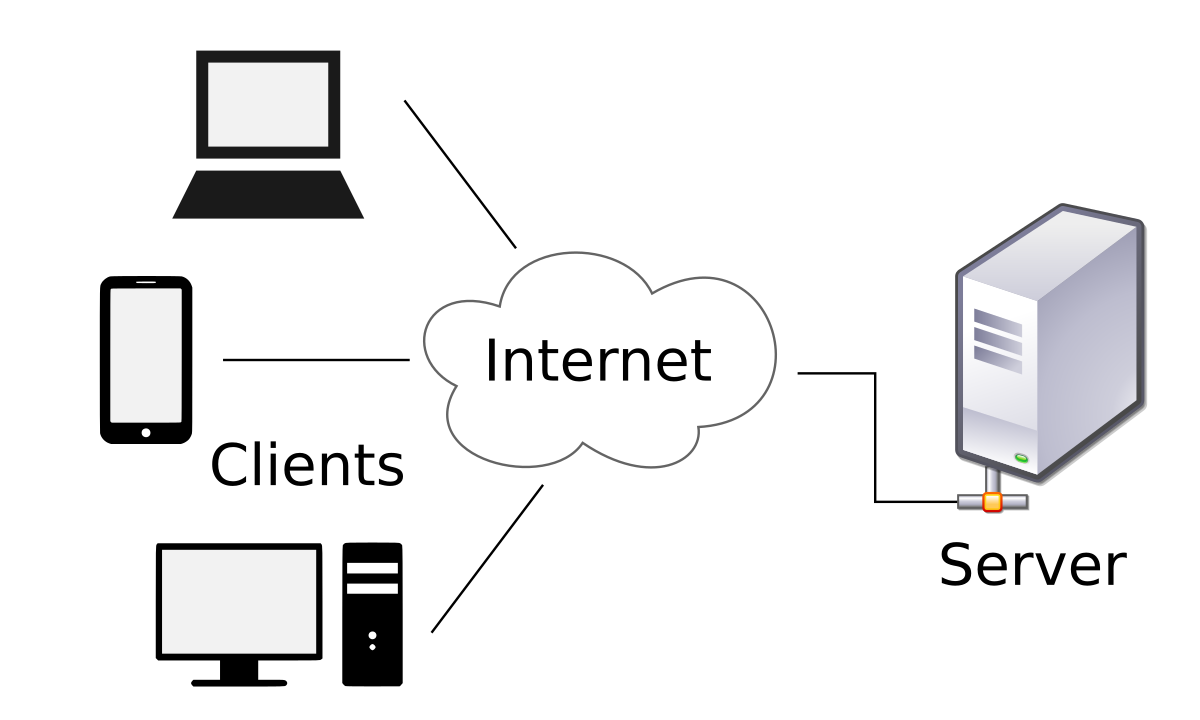
\includegraphics[width=0.5\textwidth]{figures/client-server.png}
	\caption{Arquitectura Cliente-Servidor.}
	\label{fig:client-server}
\end{figure}

\subsection{Lenguaje de programación}
Se utilizará Python como lenguaje de programación. Python ha sido uno de los lenguajes más utilizados a lo largo de estos años,
es un lenguaje interpretado y es versátil puesto que no requiere de un sistema operativo en específico para poder ser ejecutado. Además,
en él se han programado muchas bibliotecas que contienen funciones que sirven para la Ciencia de Datos, el procesamiento y visualización de datos.
Todas ellas serán utilizadas de forma nativa, sin embargo, para la construcción de la parte gráfica de la herramienta se utilizará un Framework
llamado Streamlit.


\subsection{Streamlit}
Streamlit es un Framework que tiene una gran cantidad de herramientas visuales como lo son: barras de progreso, gráficas, botones, barras de navegación,
textos información, de logro, de advertencia, de error, tablas y de impresión de código. Además es responsivo, por lo que independientemente del dispositivo
desde el que se ingrese la información de visualizará de forma correcta. Streamlit muestra cualquier otra información generada desde Python, lo cual facilita
el uso de bibliotecas nativas.


\subsection{Bibliotecas utilizadas en Python}
Para poder implementar el código en Python, se utilizaron las siguientes bibliotecas (si el usuario utiliza el software de forma local requerirá instalarlas):
\begin{itemize}
	\item numpy: creación de vectores y matrices multidimensionales.
	\item pandas: manipulación y análisis de datos.
	\item seaborn: visualización de datos estadísticos. 
	\item scipy: ecosistema para matemáticas, ciencia  e ingeniería
	\item sklearn: herramientas para herramientas de análisis de datos predictivo.
	\item io: manejo de interrupciones del sistema.
	\item SessionState: guardado del estado del sistema.
	\item kneed: método del codo.
	\item mpl\_toolkits: graficación en 3D.
	\item time: manipulación del tiempo.
	\item math: fórmulas matemáticas.
\end{itemize}

\subsection{Diagrama de casos de uso}

A continuación se muestra el diagrama de casos de uso (UML), que permite visualizar la interacción del usuario con
el sistema.

\begin{figure}[!htb]
	\centering
	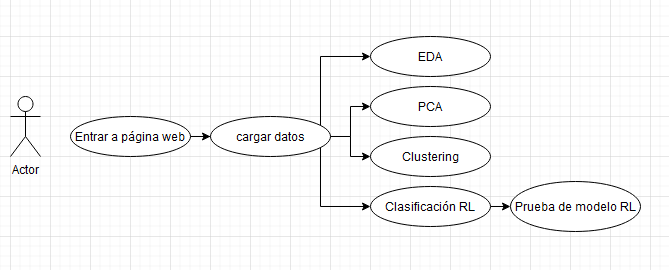
\includegraphics[width=0.4\textwidth]{figures/UML.png}
	\caption{UML.}
	\label{fig:UML}
\end{figure}

\subsection{Diagrama de procesos}

El diagrama de procesos, explica de forma detallada las funciones del sistema y del usuario. Este diagrama da una noción de las instrucciones
que el usuario debe seguir y el papel que juega para el correcto funcionamiento del sistema.
\begin{figure}[!htb]
	\centering
	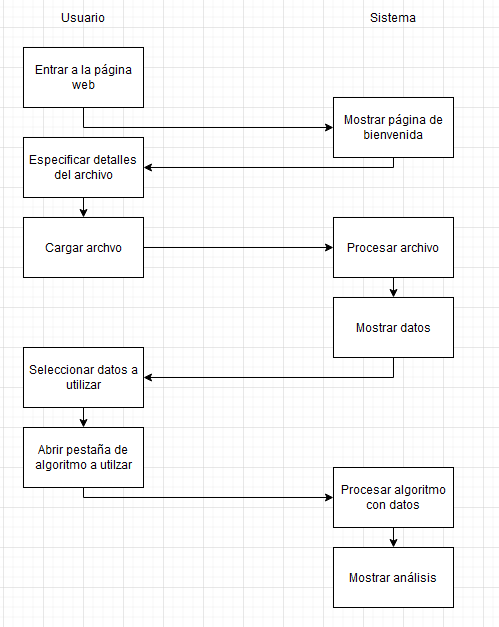
\includegraphics[width=0.4\textwidth]{figures/DDP.png}
	\caption{Diagrama de procesos.}
	\label{fig:diagramaDeProcesos}
\end{figure}

\section{Implementación}
Se considera que Heroku es un buen host para poder alojar a la aplicación. La página donde se encontrará disponible la herramienta es:
\url{http://phmdstreamlit.herokuapp.com/} Para la demostración de la aplicación se utilizará un servidor local, esto con el fin de que 
el procesamiento de los datos sea más rápido.

\subsection{Bienvenida}

En esta página se muestra la bienvenida al usuario y se le da la instrucción de dar clic en la barra de navegación, donde posteriormente el usuario dará
clic en la opción de carga de datos para poner algún archivo que sea de su interés para analizar.
\begin{figure}[!htb]
	\centering
	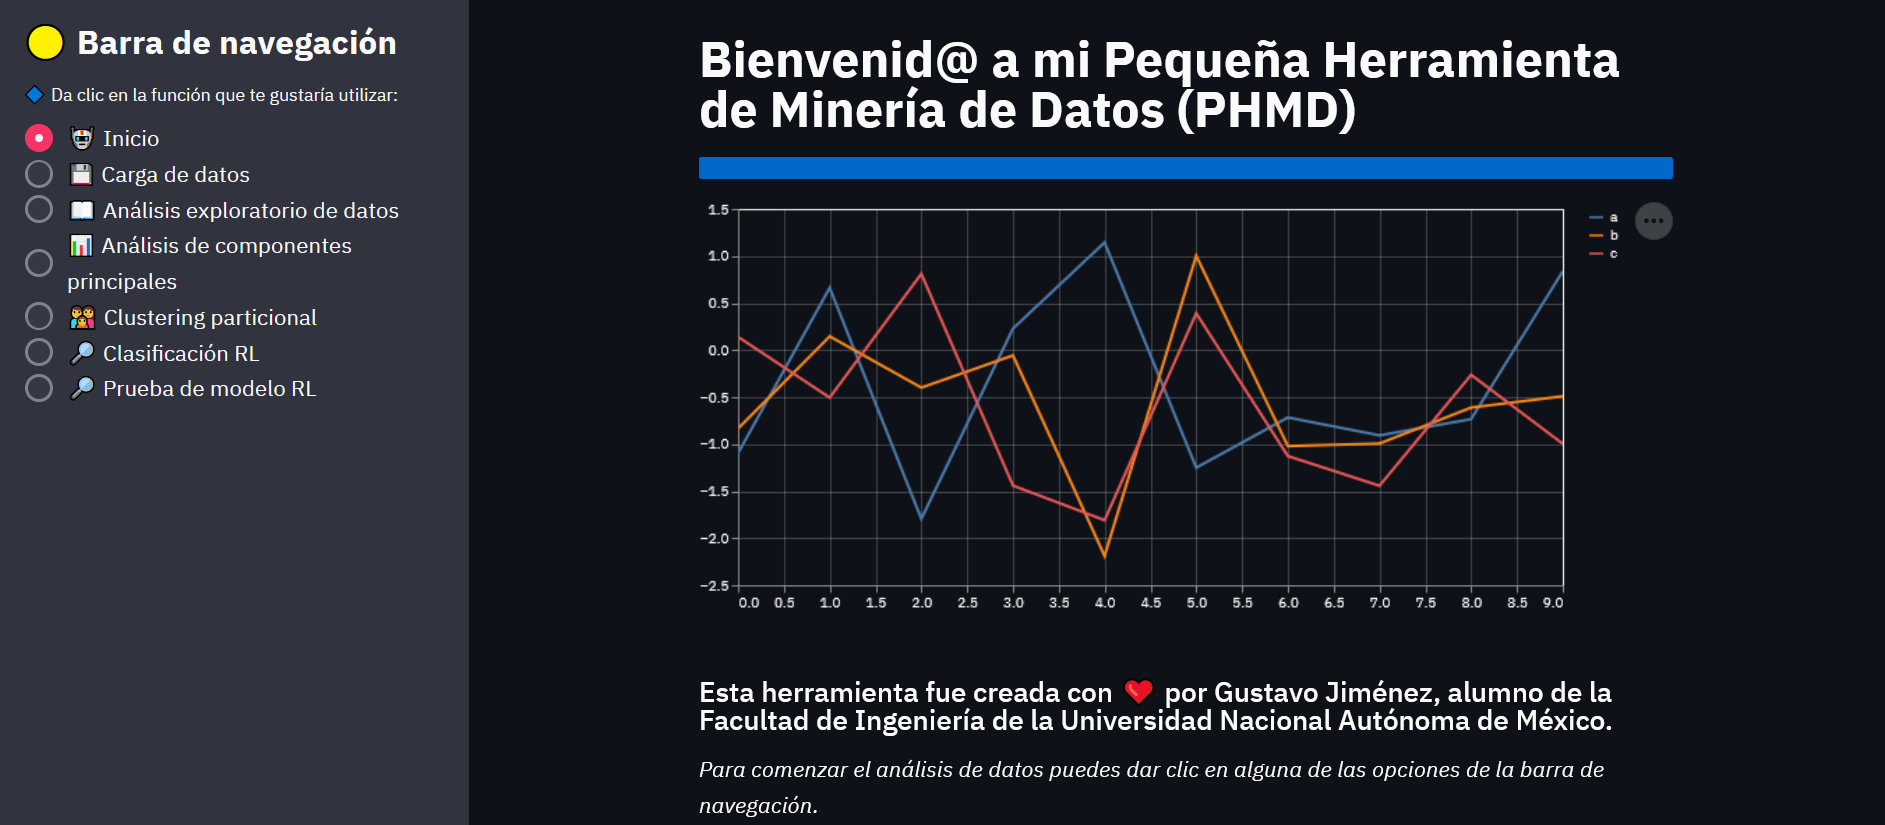
\includegraphics[width=0.7\textwidth]{figures/pagina-inicio.png}
	\caption{Página de bienvenida.}
	\label{fig:pagina-inicio}
\end{figure}

\subsection{Carga de datos}
\noindent Cuando el usuario se dirija a la pestaña de carga de datos, tendrá la opción de indicar si su archivo contiene encabezado, la separación de los datos (si es el caso) y
posteriormente, escoger el archivo con las extensiones disponibles: txt, csv y xls. Cuando se carga el archivo, se le da la posibilidad de recortar los datos por medio
de la eliminación de columnas, además se puede reemplazar algún dato en específico de alguna columna que el usuario requiera. Cabe mencionar que la interfaz muestra mensajes
de logros, advertencias y errores, con lo que se da una retroalimentación al usuario para que sepa si un proceso ha finalizado, si hay algo que considerar o si el proceso no pudo finalizar.\\
\begin{figure}[!htb]
	\centering
	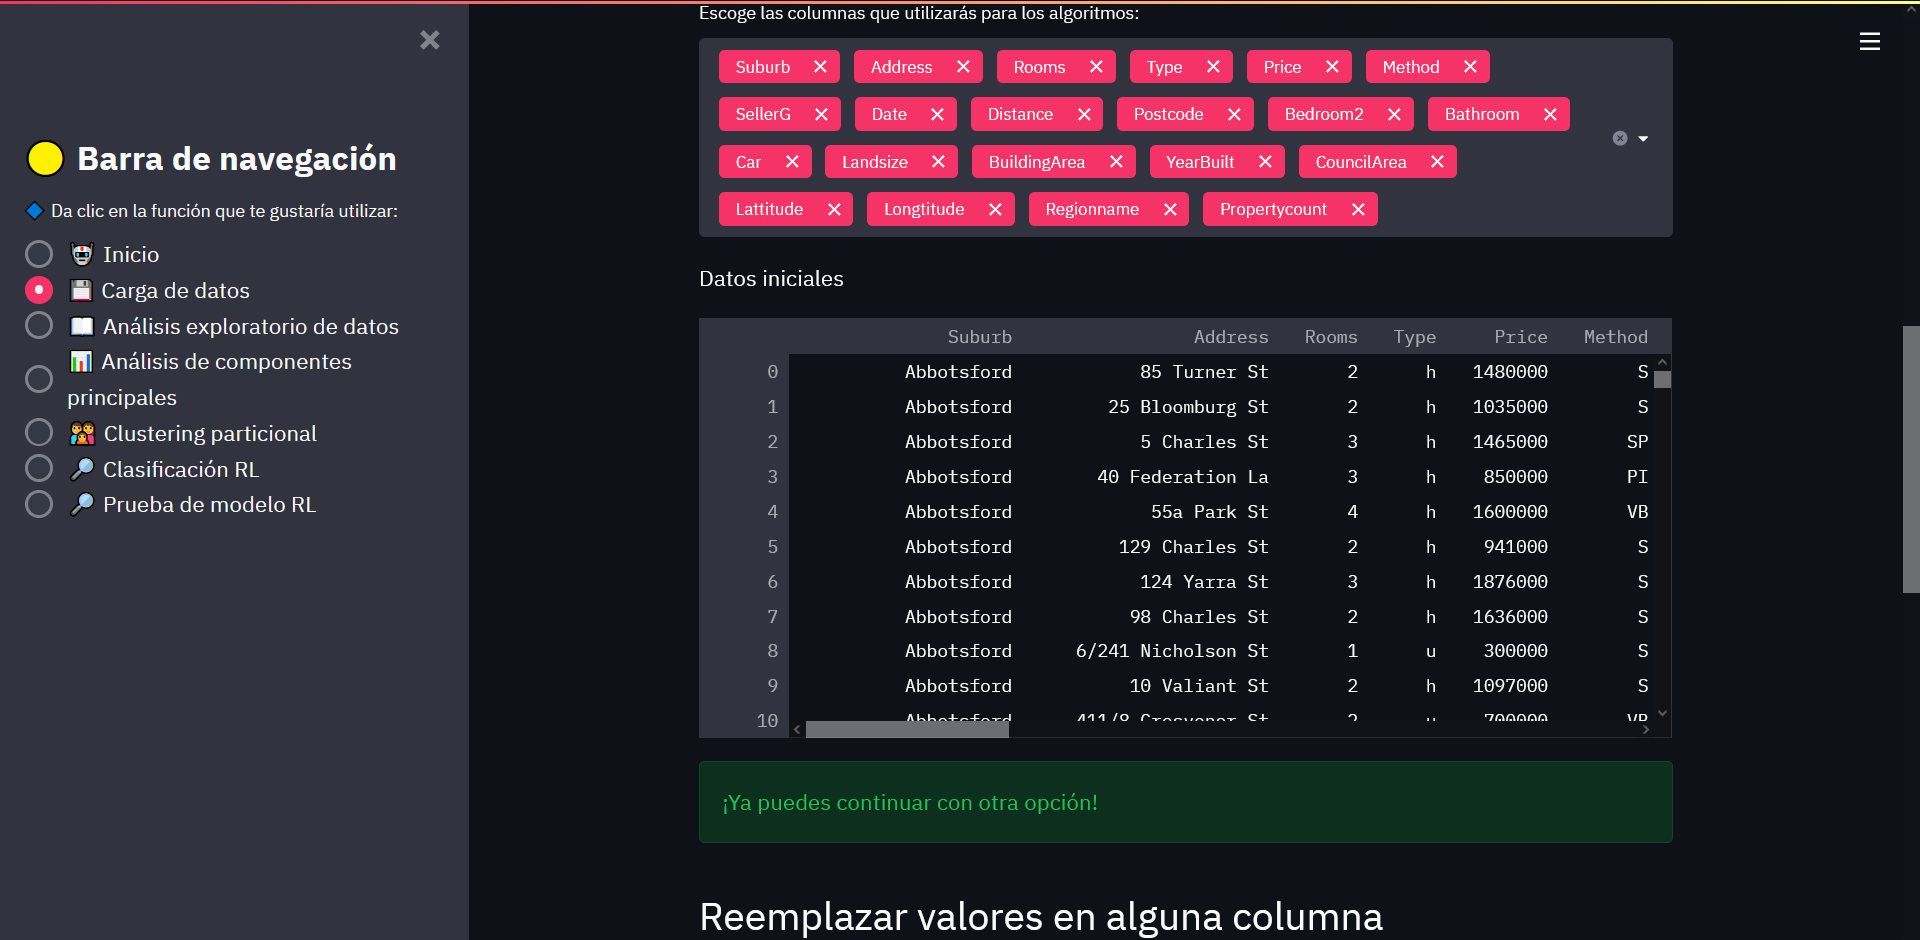
\includegraphics[width=0.5\textwidth]{figures/pagina-carga-datos.png}
	\caption{Página de carga de datos.}
	\label{fig:carga-datos}
\end{figure}

\subsection{Análisis Exploratorio de Datos}
\noindent La siguiente página es la de Análisis Exploratorio de datos. En esta página se visualiza primero el conjunto de datos con el que se trabajará, después por medio de un botón,
cuando el usuario se encuentre seguro de la información que subió, podrá iniciar la ejecución. Aquí se mostrará la descripción de los datos: sus dimensiones, los tipos de dato
de cada variable; también se grafica la distribución de cada variable para poder visualizar si hay algún sesgo en alguna de ellas; se muestra un análisis estadístico de las variables:
conteo, promedio, valores máximos y mínimos, distribución de los registros. El programa, por defecto, muestra un diagrama de cajas y bigote de las variables, lo cual facilitará
al usuario visualizar valores atípicos. Posteriormente, se muestra una distribución de aquellas variables que son categóricas. Al final del programa, se le muestra al usuario en forma de tabla
y gráfica la correlación entre las variables.

\begin{figure}[!htb]
	\centering
	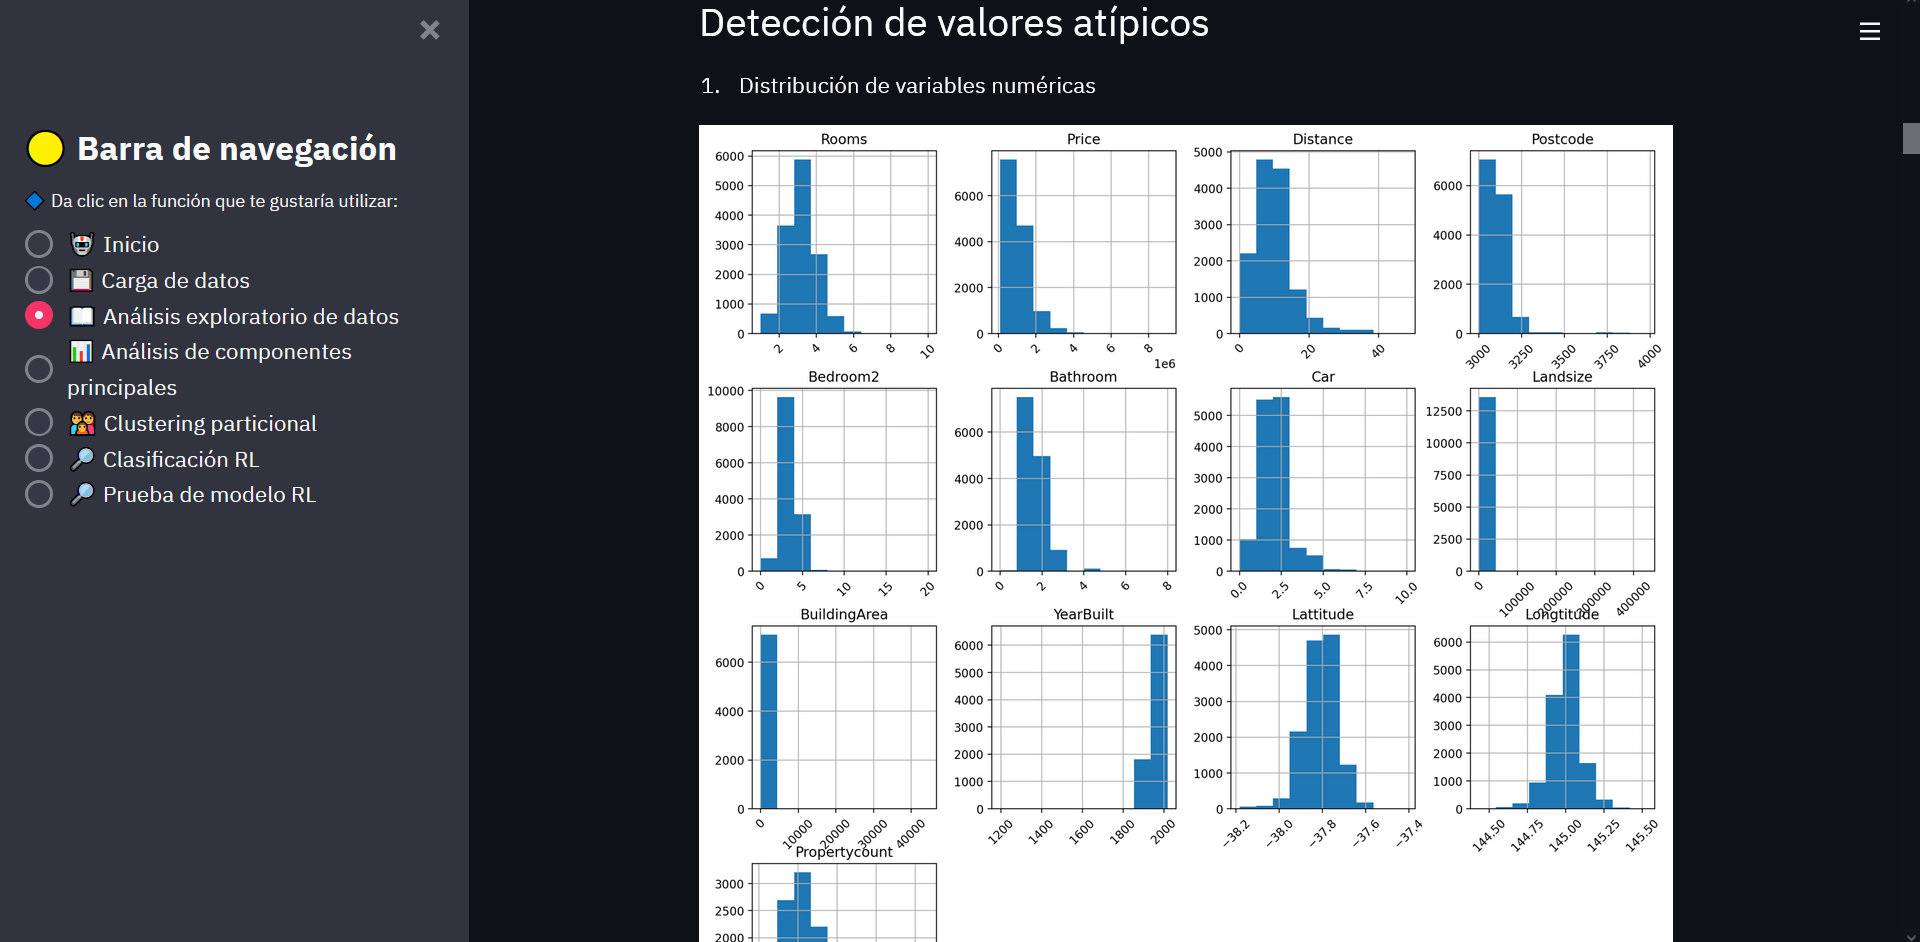
\includegraphics[width=0.5\textwidth]{figures/pagina-eda.png}
	\caption{Distribución de cada variable de un conjunto de datos.}
	\label{fig:pagina-eda}
\end{figure}

\subsection{Análisis de Componentes Principales}
\noindent La siguiente página se trata de Análisis de Componentes Principales. En ella también se visualiza el conjunto de datos con el que se hará el análisis, cuando el usuario está
listo de que sus datos son correctos, por medio del botón Iniciar ejecución comienza el análisis. Con ello, se mostrarán los renglones y columnas con los que cuenta el conjunto de datos.
Después se mostrará la normalización de los datos, una matriz de covarianzas y correlaciones, varianza y componentes. El programa extraerá los valores propios del conjunto de datos.
Posteriormente, mostrará la varianza acumulada entre componentes. Finalmente se muestran las cargas de cada variable. Este tipo de análisis es importante puesto que ayuda al usuario a
saber qué variables son las más reelevantes y cuales menos, disminuyendo problemas de dimensionalidad.

\begin{figure}[!htb]
	\centering
	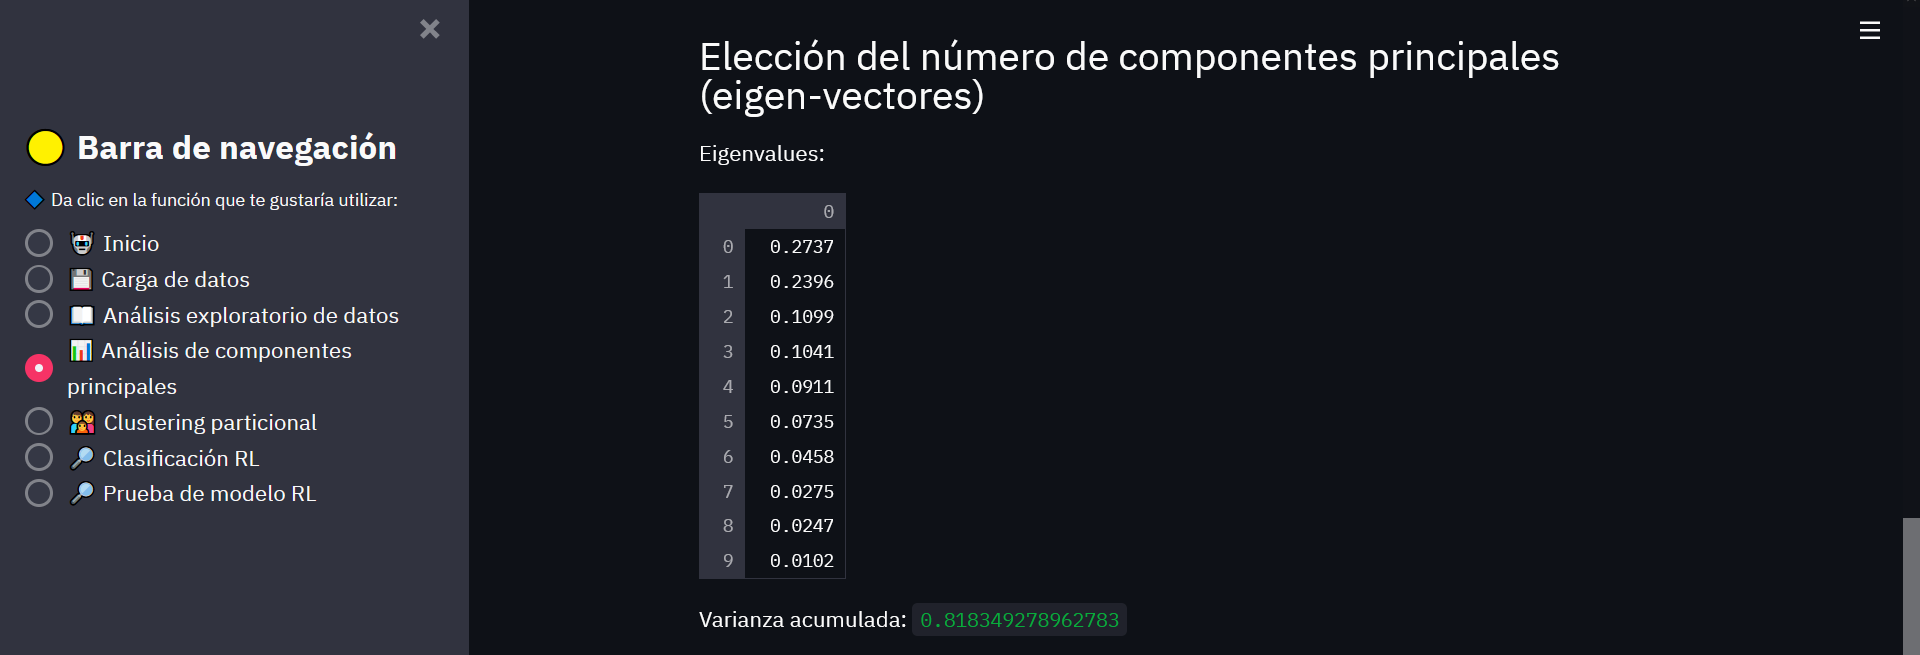
\includegraphics[width=0.5\textwidth]{figures/pagina-pca.png}
	\caption{Generación de eigen vectores.}
	\label{fig:pagina-pca}
\end{figure}

\subsection{Clustering particional}
\noindent En la página de Clustering Particional también se visualiza el conjunto de datos que se utilizará para el agrupamiento, se le permite al usuario visualizar comparación entre variables
con el fin de poder discriminar aquellas que tengan una alta similitud, después se solicita al usuario la columna principal para generar la matriz de correlaciones, cuando el usuario esté listo
dará clic en el botón de Iniciar ejecución. Después, se mostrará la matriz de correlaciones variable contra variable, la tabla con los valores numéricos y un mapa de calor. También se le muestran
al usuario las variables que está utilizando para la creación de los grupos; el programa hace una elección del número ideal de k-medias a utilzar (método del codo), muestra el número y posteriormente hace
el agrupamiento. Éste será exhibido de forma gráfica y en tabla, además se muestra la estadística de cada grupo que se creó con el fin de reconocer las características más significativas de cada
grupo. También se puede visualizar un gráfico 3D de los grupos formados y se muestra el número de registro que se encuentra más cercano al centroide. Este algoritmo es sumamente importante puesto
que de datos no etiquetados podemos pasar a datos que se encuentran agrupados por características similares, permitiendo reconocer diferencias significativas entre cada grupo de datos.

\begin{figure}[!htb]
	\centering
	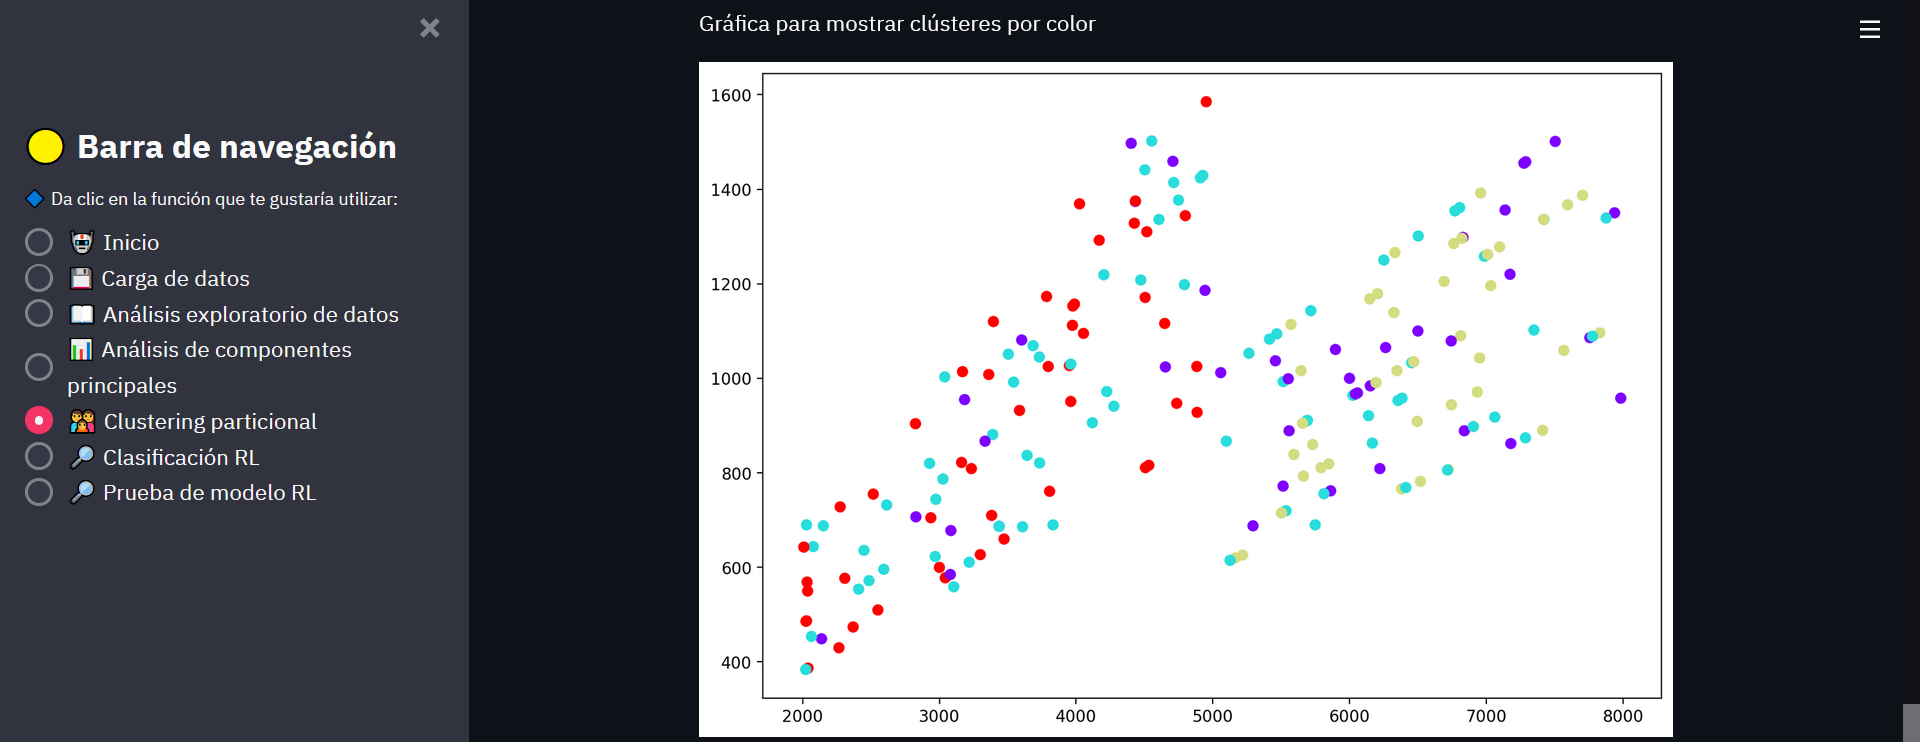
\includegraphics[width=0.6\textwidth]{figures/pagina-clustering.png}
	\caption{Grupos de un conjunto de datos.}
	\label{fig:pagina-clustering}
\end{figure}

\subsection{Clasificación RL}
\noindent En la siguiente opción se visualiza la página de Clasificación RL donde el usuario podrá visualizar el conjunto de datos con el que trabajará, puede escoger la variable predictora con la que
hará el análisis, comparar correlación entre variables, consecuentemente si se da clic en el botón de Iniciar ejecución se mostrará el análisis de los datos. El usuario puede visualizar un mapa de calor
de las correlaciones entre los datos, posteriormente se aplica el algoritmo, se le muestra al usuario el algoritmo con el que se está trabajando, las predicciones que hace el modelo y una matriz de confusión
que muestra qué tan acertivo fue el algoritmo. Al final, se muestra el intercepto y los coeficientes de cada variable, así como también la exactitud, precisión, tasa de error, sensibilidad y especificidad del modelo. \newline

\begin{figure}[!htb]
	\centering
	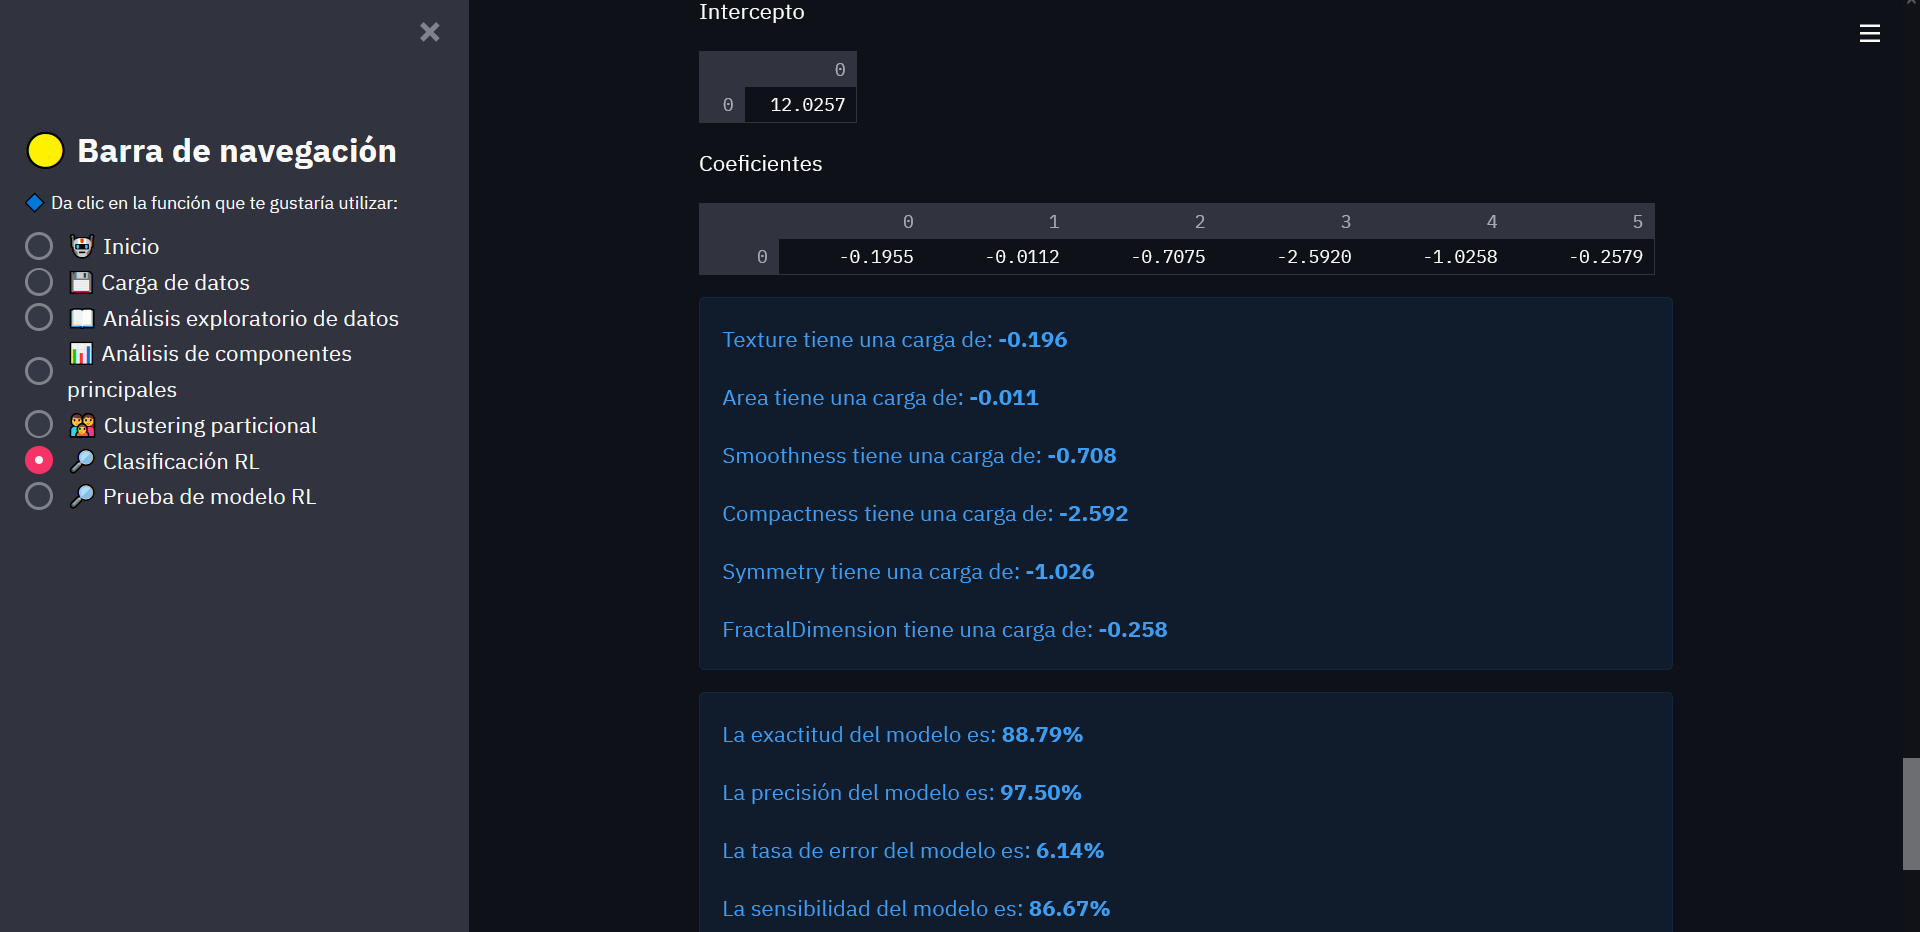
\includegraphics[width=0.5\textwidth]{figures/pagina-rl.png}
	\caption{Intercepto y coeficientes de un modelo RL.}
	\label{fig:pagina-rl}
\end{figure}

\subsection{Prueba del modelo RL}
\noindent La siguiente página sirve para el modelo RL anteriormente generado por el usuario en la pestaña de Clasificación RL, este modelo es dinámico, por lo que dependiendo del
conjunto de datos con los que se haya hecho el modelo se solicitará el número de variables para poder determinar si el valor de la variable predicha es 0 ó 1. En este caso,
el modelo fue hecho con un conjunto de datos de casos de pacientes con cáncer, dependiendo de los valores que inserte el usuario se mostrará si el cáncer que padece el paciente es
benigno o maligno.
\newline
\begin{figure}[!htb]
	\centering
	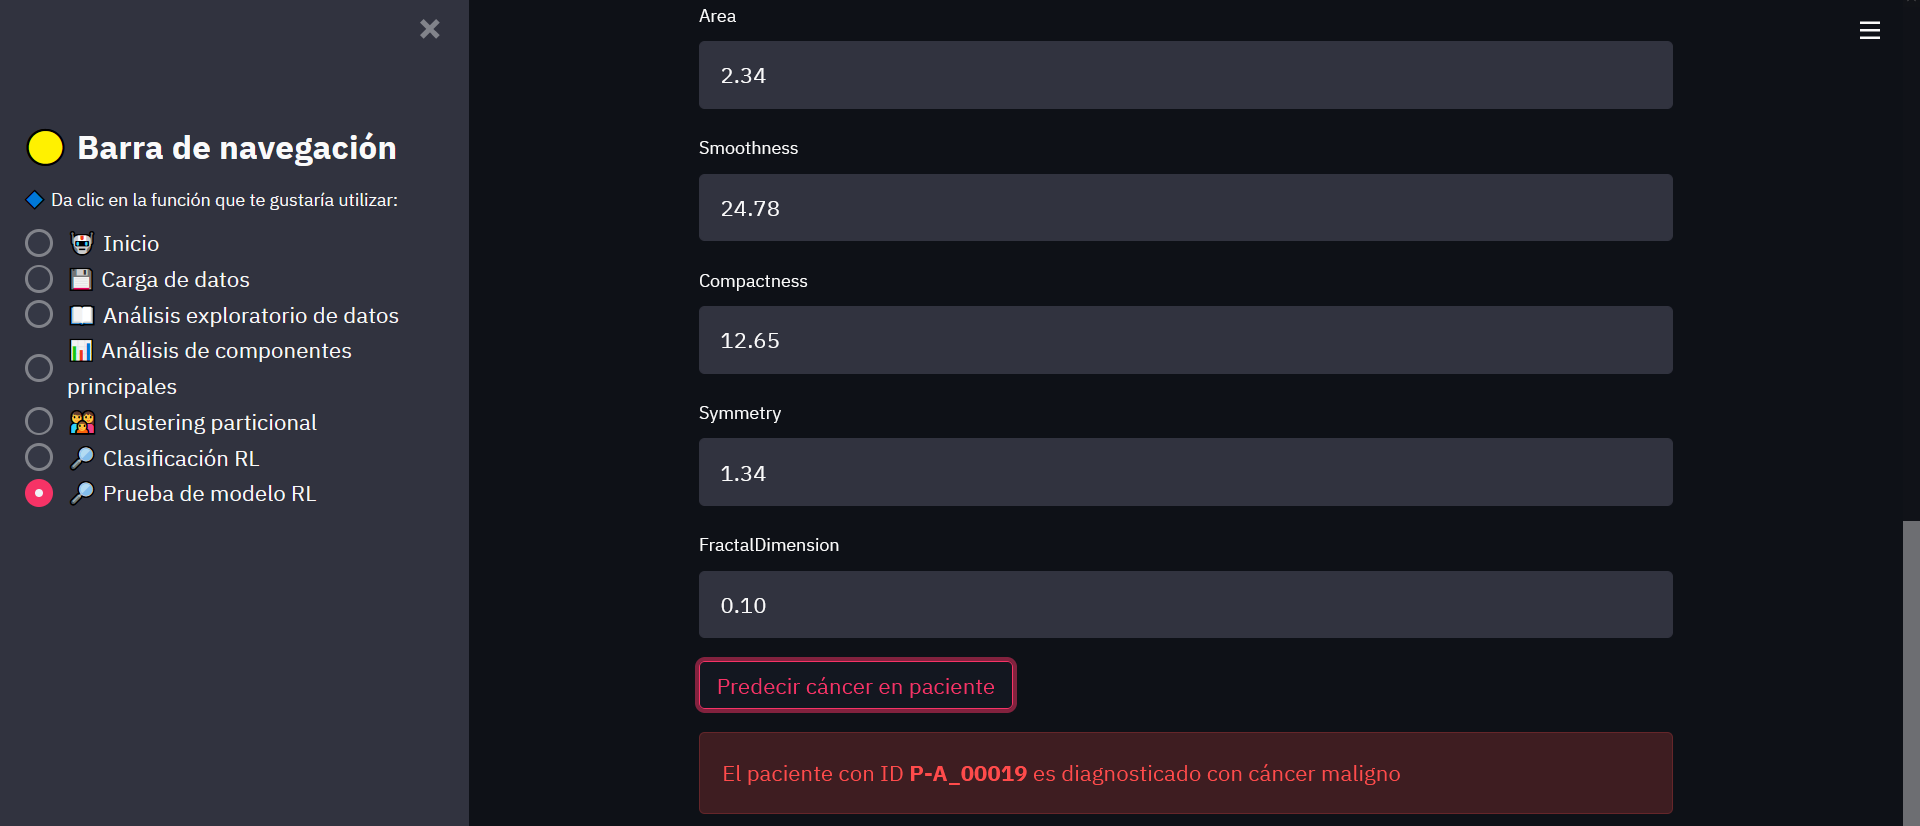
\includegraphics[width=0.5\textwidth]{figures/pagina-modelo-rl.png}
	\caption{Predicción de cáncer maligno en paciente P-A\_00019.}
	\label{fig:pagina-modelo-rl}
\end{figure}

\subsection{Observaciones}
\begin{itemize}
\item Es fundamental consideral el tamaño de los datos puesto que dependiendo de ello, se determinará el poder de procesamiento de datos que requerimos para hacer el análisis. Cuando éste 
es muy grande, es conveniente utilizar la versión del software local.
\item Streamlit es un excelente Framework para trabajar con la visualización de datos, permitiendo que el usuario se sienta cómodo por su gran facilidad de uso e intuición de manejo.
\item El usuario debe considerar hacer las modificaciones pertinentes para su conjunto de datos en la herramienta con el fin de no afectar al modelo que se genere.
\end{itemize}

\section{Conclusiones}
La Minería de Datos es un área que constantemente se requiere para descubrir información oculta de un conjunto de datos. Hay muchos aspectos que considerar para que este descubrimiento
sea del todo fructífero, estos aspectos pueden ser: el número de registros, el formato de los archivos donde esté el conjunto de datos, si las variables que se utilizan son 
nominales u ordinales, si alguna columna no es de suma relevancia, si los registros son transaccionales, si hay valores atípicos, etc. Este tipo de aspectos tienen que ser supervisados 
por un experto de tal modo que determine si el conjunto de datos es el correcto.
\newline
\newline
\noindent
Resulta necesario conocer esta área, puesto que es aplicada en muchos otros campos, proporciona una mejora en la toma de decisiones y permite ver más allá que solo datos.
Cada uno de los métodos que fueron implementados proporciona el análisis de diferentes tipos de datos, al igual que son requeridos en distintas áreas. En el
Análsis Exploratorio de Datos, se visualizó que pueden existir errores humanos que sesgan los modelos, que muchas veces los registros no se llenan de forma correcta y quedan incompletos.
Sin embargo, también resulta útil para determinar la estadística de esos datos y poder identificar frecuencia de valores. También aprendí que la multidimensionalidad puede resultar
desventajoso para el procesamiento computacional, por lo que utilizar el Análisis de Componentes Principales puede ayudar a determinar qué variables son las que más peso pueden tener
en un modelo. El Clustering es importante cuando los datos no tienen una etiqueta y por lo tanto no se puede determinar su categoría. Finalmente, la Regresión Logística ayuda a predecir
valores binarios mediante un modelo, utilizando un conjunto de datos para el entrenamiento y otro para la prueba.
\newline
\newline
\noindent
Como Ingenieros en Computación es importante aprender a hacer este tipo de análisis sin dejar de un lado que quien será el usuario también querrá saber qué es lo que sucede con los datos,
por lo que es necesario diseñar una interfaz que permita la visualización de los análisis de una forma profesional, en esta ocasión se utilizó python como lenguaje de programación principal y
el Framework Streamlit, lo cual permitió que la información y el análisis tuvieran un alcance más allá de un programador.
\newline

\section{Referencias}
\noindent 1. Mashinchi, N. (2021, 17 marzo). \textit{A quick tutorial on how to deploy your Streamlit app to Heroku.} Medium.
Recuperado 09 de agosto del 2021, de \\ \url{https://towardsdatascience.com/a-quick-tutorial-on-how-to-deploy-your-streamlit-app-to-heroku-874e1250dadd}\newline \newline
2. \textit{Welcome to Streamlit - Streamlit 0.86.0 documentation.} (2021). Streamlit. \\ Recuperado 09 de agosto de 2021, de \\
\url{https://docs.streamlit.io/en/stable/}\newline \newline
3. \textit{API reference - Streamlit 0.86.0 documentation.} (2021). Streamlit. \\ Recuperado 09 de agosto de 2021, de \\
\url{https://docs.streamlit.io/en/stable/api.html}

\end{document}